\documentclass[12pt,a4paper]{article}
\usepackage[UTF8]{ctex}
\usepackage{amsmath,amssymb,amsfonts}
\usepackage{graphicx}
\usepackage{geometry}
\usepackage{listings}
\usepackage{xcolor}
\usepackage{float}
\usepackage{booktabs}

\geometry{left=2.5cm,right=2.5cm,top=2.5cm,bottom=2.5cm}

% 定义Rust语言（listings默认不支持Rust）
\lstdefinelanguage{Rust}{
    keywords={fn, let, mut, pub, struct, impl, self, Self, if, else, match, for, while, loop, return, break, continue, use, mod, pub, crate, super, where, trait, type, const, static, ref, move, async, await, dyn, enum, true, false, Some, None, Ok, Err, Vec, Option, Result, String, bool, i32, i64, f32, f64, u8, u32, u64, usize, isize},
    keywordstyle=\color{blue}\bfseries,
    ndkeywords={println, print, format, vec, assert, assert_eq, unwrap, expect, clone, iter, map, filter, collect, push, pop, len, is_empty, abs, sqrt, sin, cos, tan, acos, to_degrees, to_radians, clamp, partial_cmp},
    ndkeywordstyle=\color{purple},
    sensitive=true,
    comment=[l]{//},
    morecomment=[s]{/*}{*/},
    commentstyle=\color{green!60!black}\itshape,
    string=[b]",
    stringstyle=\color{red},
    morestring=[b]',
}

\lstset{
    language=Rust,
    basicstyle=\ttfamily\small,
    keywordstyle=\color{blue}\bfseries,
    commentstyle=\color{green!60!black}\itshape,
    stringstyle=\color{red},
    numbers=left,
    numberstyle=\tiny\color{gray},
    frame=single,
    breaklines=true,
    showstringspaces=false,
    tabsize=4,
    captionpos=b,
    escapeinside={(*@}{@*)},
}

\title{《计算机图形学及人机交互》作业5}
\author{2023112621 程泽凯}
\date{\today}

\begin{document}

% 首页单独一页
\maketitle
\thispagestyle{empty}
\newpage

% 目录放到第二页
\tableofcontents
\thispagestyle{empty}
\newpage
\setcounter{page}{1}

\section{三维空间三角形变换}

设三维空间某三角形的三个顶点分别为$P_1(x_1,y_1,z_1)$、$P_2(x_2,y_2,z_2)$、$P_3(x_3,y_3,z_3)$。

\subsection{平移变换}

沿X轴、Y轴和Z轴分别平移$d_x$、$d_y$和$d_z$的长度。

\textbf{变换矩阵：}
\[
T = \begin{bmatrix}
1 & 0 & 0 & d_x \\
0 & 1 & 0 & d_y \\
0 & 0 & 1 & d_z \\
0 & 0 & 0 & 1
\end{bmatrix}
\]

\textbf{变换后的顶点坐标：}
\begin{align*}
P_1' &= (x_1 + d_x, y_1 + d_y, z_1 + d_z) \\
P_2' &= (x_2 + d_x, y_2 + d_y, z_2 + d_z) \\
P_3' &= (x_3 + d_x, y_3 + d_y, z_3 + d_z)
\end{align*}

\subsection{旋转变换}

\textbf{绕X轴旋转$\alpha$度的变换矩阵：}
\[
R_x(\alpha) = \begin{bmatrix}
1 & 0 & 0 & 0 \\
0 & \cos\alpha & -\sin\alpha & 0 \\
0 & \sin\alpha & \cos\alpha & 0 \\
0 & 0 & 0 & 1
\end{bmatrix}
\]

\textbf{绕Y轴旋转$\beta$度的变换矩阵：}
\[
R_y(\beta) = \begin{bmatrix}
\cos\beta & 0 & \sin\beta & 0 \\
0 & 1 & 0 & 0 \\
-\sin\beta & 0 & \cos\beta & 0 \\
0 & 0 & 0 & 1
\end{bmatrix}
\]

\textbf{绕Z轴旋转$\theta$度的变换矩阵：}
\[
R_z(\theta) = \begin{bmatrix}
\cos\theta & -\sin\theta & 0 & 0 \\
\sin\theta & \cos\theta & 0 & 0 \\
0 & 0 & 1 & 0 \\
0 & 0 & 0 & 1
\end{bmatrix}
\]

\textbf{复合旋转变换矩阵：}
\[
R = R_z(\theta) \cdot R_y(\beta) \cdot R_x(\alpha)
\]

\textbf{复合旋转矩阵展开：}

设 $c_\alpha = \cos\alpha$, $s_\alpha = \sin\alpha$, $c_\beta = \cos\beta$, $s_\beta = \sin\beta$, $c_\theta = \cos\theta$, $s_\theta = \sin\theta$，则：
\[
R = \begin{bmatrix}
c_\theta c_\beta & c_\theta s_\beta s_\alpha - s_\theta c_\alpha & c_\theta s_\beta c_\alpha + s_\theta s_\alpha \\
s_\theta c_\beta & s_\theta s_\beta s_\alpha + c_\theta c_\alpha & s_\theta s_\beta c_\alpha - c_\theta s_\alpha \\
-s_\beta & c_\beta s_\alpha & c_\beta c_\alpha
\end{bmatrix}
\]

即：
\begin{align*}
r_{11} &= \cos\theta\cos\beta \\
r_{12} &= \cos\theta\sin\beta\sin\alpha - \sin\theta\cos\alpha \\
r_{13} &= \cos\theta\sin\beta\cos\alpha + \sin\theta\sin\alpha \\
r_{21} &= \sin\theta\cos\beta \\
r_{22} &= \sin\theta\sin\beta\sin\alpha + \cos\theta\cos\alpha \\
r_{23} &= \sin\theta\sin\beta\cos\alpha - \cos\theta\sin\alpha \\
r_{31} &= -\sin\beta \\
r_{32} &= \cos\beta\sin\alpha \\
r_{33} &= \cos\beta\cos\alpha
\end{align*}

\textbf{变换后的顶点坐标：}
对于任意点$P_i(x_i, y_i, z_i)$，变换后的坐标为：
\[
\begin{bmatrix} x_i' \\ y_i' \\ z_i' \\ 1 \end{bmatrix} = R \cdot \begin{bmatrix} x_i \\ y_i \\ z_i \\ 1 \end{bmatrix}
\]

变换后各顶点坐标为：
\begin{align*}
P_1' &= (r_{11}x_1 + r_{12}y_1 + r_{13}z_1, \; r_{21}x_1 + r_{22}y_1 + r_{23}z_1, \; r_{31}x_1 + r_{32}y_1 + r_{33}z_1) \\
P_2' &= (r_{11}x_2 + r_{12}y_2 + r_{13}z_2, \; r_{21}x_2 + r_{22}y_2 + r_{23}z_2, \; r_{31}x_2 + r_{32}y_2 + r_{33}z_2) \\
P_3' &= (r_{11}x_3 + r_{12}y_3 + r_{13}z_3, \; r_{21}x_3 + r_{22}y_3 + r_{23}z_3, \; r_{31}x_3 + r_{32}y_3 + r_{33}z_3)
\end{align*}

\subsection{以P1为中心的缩放变换}

在保持$P_1$点位置不变的情况下，将三角形三条边的边长分别放大$s$倍。

\textbf{变换步骤：}
\begin{enumerate}
    \item 将$P_1$平移到原点
    \item 进行缩放变换
    \item 将原点平移回$P_1$
\end{enumerate}

\textbf{变换矩阵：}
\[
S_{P_1} = T(x_1, y_1, z_1) \cdot S(s) \cdot T(-x_1, -y_1, -z_1)
\]

其中：
\[
T(x_1, y_1, z_1) = \begin{bmatrix}
1 & 0 & 0 & x_1 \\
0 & 1 & 0 & y_1 \\
0 & 0 & 1 & z_1 \\
0 & 0 & 0 & 1
\end{bmatrix}, \quad
S(s) = \begin{bmatrix}
s & 0 & 0 & 0 \\
0 & s & 0 & 0 \\
0 & 0 & s & 0 \\
0 & 0 & 0 & 1
\end{bmatrix}
\]

\textbf{复合变换矩阵：}
\[
S_{P_1} = \begin{bmatrix}
s & 0 & 0 & x_1(1-s) \\
0 & s & 0 & y_1(1-s) \\
0 & 0 & s & z_1(1-s) \\
0 & 0 & 0 & 1
\end{bmatrix}
\]

\textbf{变换后的顶点坐标：}
\begin{align*}
P_1' &= (x_1, y_1, z_1) \\
P_2' &= (x_1 + s(x_2 - x_1), y_1 + s(y_2 - y_1), z_1 + s(z_2 - z_1)) \\
P_3' &= (x_1 + s(x_3 - x_1), y_1 + s(y_3 - y_1), z_1 + s(z_3 - z_1))
\end{align*}

\subsection{依次完成平移、旋转、缩放操作}

依次完成(1)(2)(3)步的操作。

\textbf{复合变换矩阵：}
\[
M = S_{P_1'} \cdot R \cdot T
\]

其中$P_1' = (x_1 + d_x, y_1 + d_y, z_1 + d_z)$是平移后$P_1$的位置。

注意：由于缩放是以平移后的$P_1'$为中心，所以需要先计算平移后的位置。

\textbf{完整的复合变换矩阵：}
\[
M = T(P_1') \cdot S(s) \cdot T(-P_1') \cdot R_z(\theta) \cdot R_y(\beta) \cdot R_x(\alpha) \cdot T(d_x, d_y, d_z)
\]

\textbf{变换后的顶点坐标：}
\[
\begin{bmatrix} x_i'' \\ y_i'' \\ z_i'' \\ 1 \end{bmatrix} = M \cdot \begin{bmatrix} x_i \\ y_i \\ z_i \\ 1 \end{bmatrix}
\]

设$P_1' = (x_1+d_x, y_1+d_y, z_1+d_z)$为平移后$P_1$的位置，$R$为复合旋转矩阵（元素$r_{ij}$如1.2节所述）。

\textbf{变换过程分析：}
\begin{enumerate}
    \item 平移后：$P_i^{(1)} = P_i + (d_x, d_y, d_z)$
    \item 旋转后：$P_i^{(2)} = R \cdot P_i^{(1)}$
    \item 以$P_1^{(2)}$为中心缩放后：$P_i'' = P_1^{(2)} + s(P_i^{(2)} - P_1^{(2)})$
\end{enumerate}

由于$P_1$经过旋转后位置改变，设$P_1^{(2)} = R \cdot P_1' = R \cdot (P_1 + (d_x,d_y,d_z)^T)$。

\textbf{变换后各顶点坐标：}
\begin{align*}
P_1'' &= R \cdot (P_1 + (d_x, d_y, d_z)^T) \\
      &= (r_{11}(x_1+d_x) + r_{12}(y_1+d_y) + r_{13}(z_1+d_z), \\
      &\quad r_{21}(x_1+d_x) + r_{22}(y_1+d_y) + r_{23}(z_1+d_z), \\
      &\quad r_{31}(x_1+d_x) + r_{32}(y_1+d_y) + r_{33}(z_1+d_z))
\end{align*}

\begin{align*}
P_2'' &= P_1'' + s \cdot (R \cdot (P_2 + (d_x,d_y,d_z)^T) - P_1'') \\
      &= P_1'' + s \cdot R \cdot (P_2 - P_1)
\end{align*}

\begin{align*}
P_3'' &= P_1'' + s \cdot (R \cdot (P_3 + (d_x,d_y,d_z)^T) - P_1'') \\
      &= P_1'' + s \cdot R \cdot (P_3 - P_1)
\end{align*}

展开$P_2''$的各分量：
\begin{align*}
x_2'' &= x_1'' + s \cdot [r_{11}(x_2-x_1) + r_{12}(y_2-y_1) + r_{13}(z_2-z_1)] \\
y_2'' &= y_1'' + s \cdot [r_{21}(x_2-x_1) + r_{22}(y_2-y_1) + r_{23}(z_2-z_1)] \\
z_2'' &= z_1'' + s \cdot [r_{31}(x_2-x_1) + r_{32}(y_2-y_1) + r_{33}(z_2-z_1)]
\end{align*}

$P_3''$同理可得。

\subsection{绕任意轴旋转}

以空间某线段$P_4(x_4,y_4,z_4)P_5(x_5,y_5,z_5)$为轴旋转$\alpha$度角。

\textbf{算法步骤：}
\begin{enumerate}
    \item 将$P_4$平移到原点
    \item 将旋转轴旋转到与Z轴重合
    \item 绕Z轴旋转$\alpha$度
    \item 将旋转轴旋转回原来的方向
    \item 将原点平移回$P_4$
\end{enumerate}

\textbf{设旋转轴方向向量：}
\[
\vec{v} = (a, b, c) = \frac{(x_5-x_4, y_5-y_4, z_5-z_4)}{|(x_5-x_4, y_5-y_4, z_5-z_4)|}
\]

\textbf{将旋转轴旋转到Z轴的变换：}

首先绕X轴旋转，使旋转轴落在XZ平面：
\[
d = \sqrt{b^2 + c^2}
\]
\[
R_x = \begin{bmatrix}
1 & 0 & 0 & 0 \\
0 & c/d & -b/d & 0 \\
0 & b/d & c/d & 0 \\
0 & 0 & 0 & 1
\end{bmatrix}
\]

然后绕Y轴旋转，使旋转轴与Z轴重合：
\[
R_y = \begin{bmatrix}
d & 0 & -a & 0 \\
0 & 1 & 0 & 0 \\
a & 0 & d & 0 \\
0 & 0 & 0 & 1
\end{bmatrix}
\]

\textbf{完整的变换矩阵：}
\[
M_{axis} = T(x_4, y_4, z_4) \cdot R_x^{-1} \cdot R_y^{-1} \cdot R_z(\alpha) \cdot R_y \cdot R_x \cdot T(-x_4, -y_4, -z_4)
\]

\textbf{使用Rodrigues旋转公式的等价表示：}

设单位旋转轴为$\vec{k} = (k_x, k_y, k_z)$，旋转角度为$\alpha$，则旋转矩阵为：
\[
R = I + \sin\alpha \cdot K + (1-\cos\alpha) \cdot K^2
\]

其中$K$是反对称矩阵：
\[
K = \begin{bmatrix}
0 & -k_z & k_y \\
k_z & 0 & -k_x \\
-k_y & k_x & 0
\end{bmatrix}
\]

\textbf{展开后的旋转矩阵：}
\[
R = \begin{bmatrix}
\cos\alpha + k_x^2(1-\cos\alpha) & k_xk_y(1-\cos\alpha) - k_z\sin\alpha & k_xk_z(1-\cos\alpha) + k_y\sin\alpha \\
k_yk_x(1-\cos\alpha) + k_z\sin\alpha & \cos\alpha + k_y^2(1-\cos\alpha) & k_yk_z(1-\cos\alpha) - k_x\sin\alpha \\
k_zk_x(1-\cos\alpha) - k_y\sin\alpha & k_zk_y(1-\cos\alpha) + k_x\sin\alpha & \cos\alpha + k_z^2(1-\cos\alpha)
\end{bmatrix}
\]

\textbf{完整的齐次变换矩阵：}
\[
M_{axis} = T(P_4) \cdot \begin{bmatrix} R & 0 \\ 0 & 1 \end{bmatrix} \cdot T(-P_4)
\]

\textbf{变换后的顶点坐标：}
\[
\begin{bmatrix} x_i' \\ y_i' \\ z_i' \\ 1 \end{bmatrix} = M_{axis} \cdot \begin{bmatrix} x_i \\ y_i \\ z_i \\ 1 \end{bmatrix}
\]

展开后，设$\vec{p} = P_i - P_4 = (x_i-x_4, y_i-y_4, z_i-z_4)$，则：
\[
P_i' = P_4 + R \cdot \vec{p}
\]

即变换后各顶点坐标为：
\begin{align*}
P_1' &= (x_4 + R_{11}(x_1-x_4) + R_{12}(y_1-y_4) + R_{13}(z_1-z_4), \\
     &\quad y_4 + R_{21}(x_1-x_4) + R_{22}(y_1-y_4) + R_{23}(z_1-z_4), \\
     &\quad z_4 + R_{31}(x_1-x_4) + R_{32}(y_1-y_4) + R_{33}(z_1-z_4))
\end{align*}

\begin{align*}
P_2' &= (x_4 + R_{11}(x_2-x_4) + R_{12}(y_2-y_4) + R_{13}(z_2-z_4), \\
     &\quad y_4 + R_{21}(x_2-x_4) + R_{22}(y_2-y_4) + R_{23}(z_2-z_4), \\
     &\quad z_4 + R_{31}(x_2-x_4) + R_{32}(y_2-y_4) + R_{33}(z_2-z_4))
\end{align*}

\begin{align*}
P_3' &= (x_4 + R_{11}(x_3-x_4) + R_{12}(y_3-y_4) + R_{13}(z_3-z_4), \\
     &\quad y_4 + R_{21}(x_3-x_4) + R_{22}(y_3-y_4) + R_{23}(z_3-z_4), \\
     &\quad z_4 + R_{31}(x_3-x_4) + R_{32}(y_3-y_4) + R_{33}(z_3-z_4))
\end{align*}

其中$R_{ij}$为Rodrigues旋转矩阵的元素：
\begin{align*}
R_{11} &= \cos\alpha + k_x^2(1-\cos\alpha) \\
R_{12} &= k_xk_y(1-\cos\alpha) - k_z\sin\alpha \\
R_{13} &= k_xk_z(1-\cos\alpha) + k_y\sin\alpha \\
R_{21} &= k_yk_x(1-\cos\alpha) + k_z\sin\alpha \\
R_{22} &= \cos\alpha + k_y^2(1-\cos\alpha) \\
R_{23} &= k_yk_z(1-\cos\alpha) - k_x\sin\alpha \\
R_{31} &= k_zk_x(1-\cos\alpha) - k_y\sin\alpha \\
R_{32} &= k_zk_y(1-\cos\alpha) + k_x\sin\alpha \\
R_{33} &= \cos\alpha + k_z^2(1-\cos\alpha)
\end{align*}

其中单位旋转轴$\vec{k} = (k_x, k_y, k_z)$由$P_4P_5$方向确定：
\[
k_x = \frac{x_5-x_4}{L}, \quad k_y = \frac{y_5-y_4}{L}, \quad k_z = \frac{z_5-z_4}{L}
\]
\[
L = \sqrt{(x_5-x_4)^2 + (y_5-y_4)^2 + (z_5-z_4)^2}
\]

\newpage
\section{矢量长度与夹角计算}

\subsection{问题描述}
已知三维空间中矢量$\vec{u}=(u_x,u_y,u_z)$和$\vec{v}=(v_x,v_y,v_z)$，求这两条矢量的长度以及它们之间夹角大小。

\subsection{算法输入}
\begin{itemize}
    \item 三维矢量 $\vec{u} = (u_x, u_y, u_z)$
    \item 三维矢量 $\vec{v} = (v_x, v_y, v_z)$
\end{itemize}

\subsection{算法输出}
\begin{itemize}
    \item 矢量 $\vec{u}$ 的长度 $|\vec{u}|$
    \item 矢量 $\vec{v}$ 的长度 $|\vec{v}|$
    \item 两矢量的夹角 $\theta$（弧度或角度）
\end{itemize}

\subsection{算法流程}
\begin{enumerate}
    \item 计算矢量 $\vec{u}$ 的长度：$|\vec{u}| = \sqrt{u_x^2 + u_y^2 + u_z^2}$
    \item 计算矢量 $\vec{v}$ 的长度：$|\vec{v}| = \sqrt{v_x^2 + v_y^2 + v_z^2}$
    \item 计算两矢量的点积：$\vec{u} \cdot \vec{v} = u_x v_x + u_y v_y + u_z v_z$
    \item 计算夹角余弦值：$\cos\theta = \frac{\vec{u} \cdot \vec{v}}{|\vec{u}| \cdot |\vec{v}|}$
    \item 通过反余弦函数求夹角：$\theta = \arccos(\cos\theta)$
    \item 如需角度制，转换：$\theta_{deg} = \theta \times \frac{180}{\pi}$
\end{enumerate}

\subsection{数学原理}
\textbf{矢量长度（欧几里得范数）：}
\[
|\vec{u}| = \sqrt{u_x^2 + u_y^2 + u_z^2}
\]

\textbf{矢量夹角（基于点积定义）：}
\[
\cos\theta = \frac{\vec{u} \cdot \vec{v}}{|\vec{u}| \cdot |\vec{v}|} = \frac{u_x v_x + u_y v_y + u_z v_z}{|\vec{u}| \cdot |\vec{v}|}
\]

\subsection{Rust代码实现}

\begin{lstlisting}
#[derive(Debug, Clone, Copy)]
pub struct Vec3 { pub x: f64, pub y: f64, pub z: f64 }

impl Vec3 {
    pub fn new(x: f64, y: f64, z: f64) -> Self { Vec3 { x, y, z } }

    pub fn length(&self) -> f64 {
        (self.x * self.x + self.y * self.y + self.z * self.z).sqrt()
    }

    pub fn dot(&self, other: &Vec3) -> f64 {
        self.x * other.x + self.y * other.y + self.z * other.z
    }

    pub fn angle_with(&self, other: &Vec3) -> f64 {
        let len_product = self.length() * other.length();
        if len_product < 1e-10 { return 0.0; }
        let cos_theta = (self.dot(other) / len_product).clamp(-1.0, 1.0);
        cos_theta.acos()
    }

    pub fn angle_degrees(&self, other: &Vec3) -> f64 {
        self.angle_with(other).to_degrees()
    }
}

fn main() {
    let u = Vec3::new(3.0, -1.0, 4.0);
    let v = Vec3::new(2.0, 5.0, -2.0);

    println!("给定两个三维向量:");
    println!("  u = ({}, {}, {})", u.x, u.y, u.z);
    println!("  v = ({}, {}, {})", v.x, v.y, v.z);

    let len_u = u.length();
    let len_v = v.length();
    let dot_val = u.dot(&v);
    let cos_theta = dot_val / (len_u * len_v);

    println!(">>> |u| = sqrt({}+{}+{}) = {:.4}", 
             u.x*u.x, u.y*u.y, u.z*u.z, len_u);
    println!(">>> |v| = sqrt({}+{}+{}) = {:.4}", 
             v.x*v.x, v.y*v.y, v.z*v.z, len_v);
    println!(">>> u·v = {} + {} + {} = {}", 
             u.x*v.x, u.y*v.y, u.z*v.z, dot_val);
    println!(">>> cosθ = {}/{:.4} = {:.6}", dot_val, len_u*len_v, cos_theta);
    println!(">>> θ = {:.4} rad = {:.2}°", 
             u.angle_with(&v), u.angle_degrees(&v));
}
\end{lstlisting}

\subsection{运行结果}
\begin{verbatim}
给定两个三维向量:
  u = (3, -1, 4)
  v = (2, 5, -2)

>>> 计算向量u的模长
    |u| = √(3² + (-1)² + 4²)
        = √(9 + 1 + 16)
        = √26 ≈ 5.0990

>>> 计算向量v的模长
    |v| = √(2² + 5² + (-2)²)
        = √(4 + 25 + 4)
        = √33 ≈ 5.7446

>>> 计算点积 u·v
    u·v = (3)×(2) + (-1)×(5) + (4)×(-2)
        = 6 + (-5) + (-8)
        = -7

>>> 计算夹角θ
    cosθ = (u·v)/(|u||v|) = -7/(5.0990×5.7446)
         = -7/29.2916 = -0.238976
    θ = arccos(-0.238976)
      = 1.8121 rad = 103.83°
\end{verbatim}

\begin{figure}[H]
    \centering
    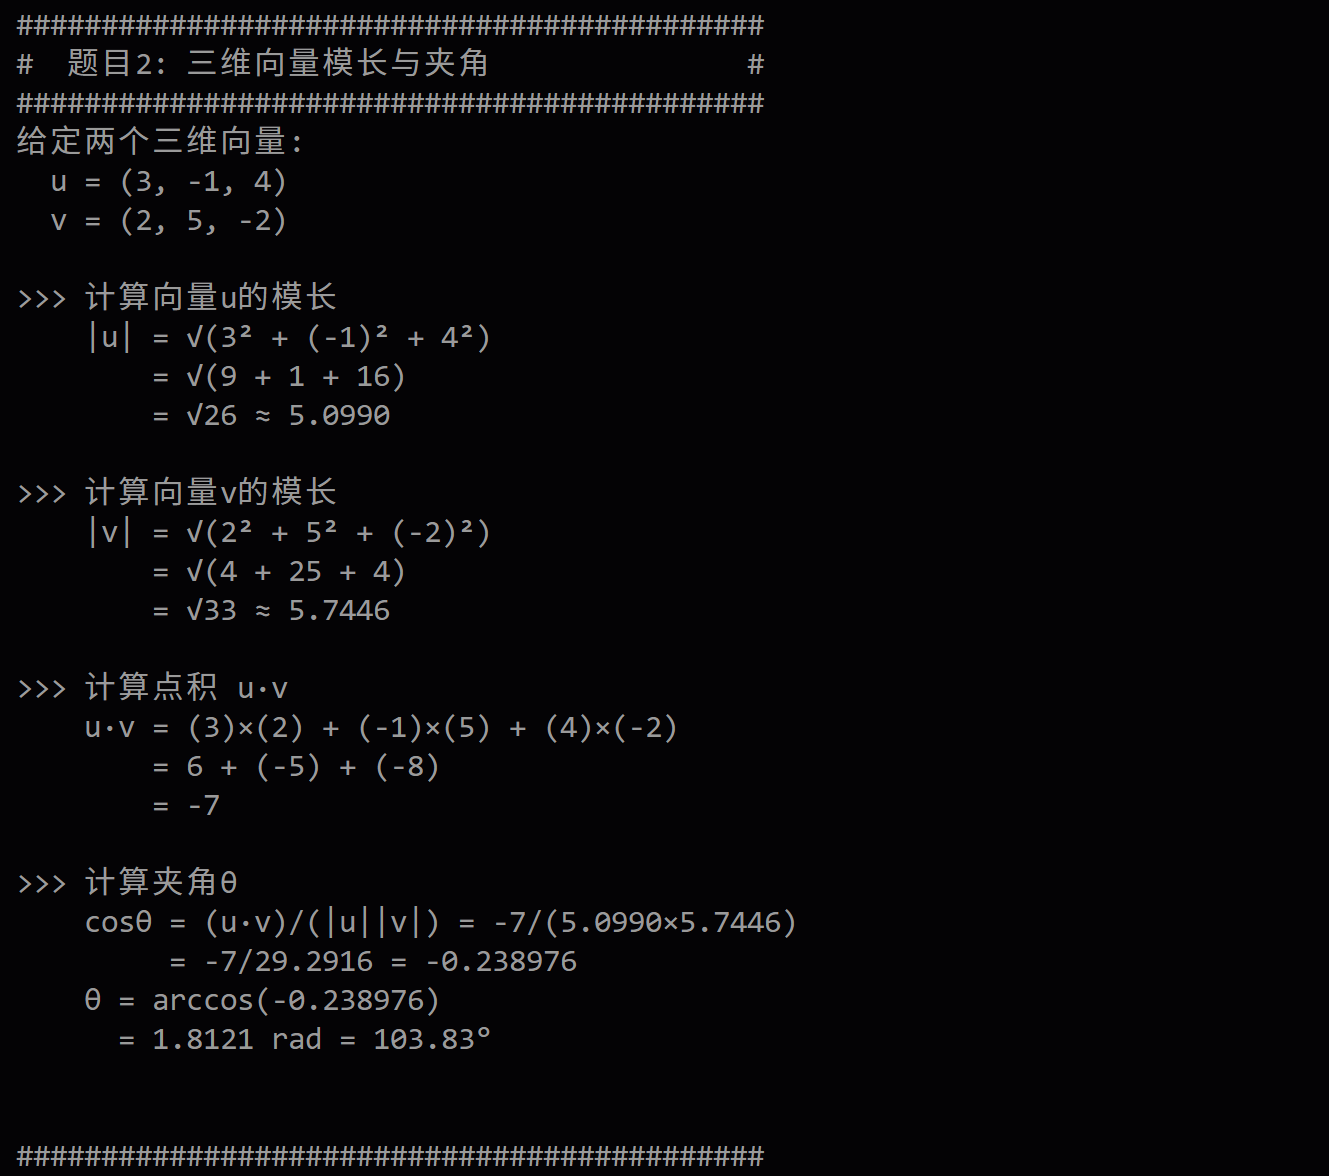
\includegraphics[width=0.8\textwidth]{vector_result.png}
    \caption{向量计算程序运行结果}
\end{figure}

\newpage
\section{中点分割裁剪算法}

\subsection{问题描述}
采用中点分割裁剪算法实现矩形窗口ABCD对线段$P_1P_2$的裁剪。

\subsection{算法输入}
\begin{itemize}
    \item 线段的两个端点：$P_1(x_1, y_1)$ 和 $P_2(x_2, y_2)$
    \item 矩形裁剪窗口：由 $(x_{min}, y_{min})$ 和 $(x_{max}, y_{max})$ 定义
\end{itemize}

\subsection{算法输出}
\begin{itemize}
    \item 若线段与窗口有交集：返回裁剪后线段的两个端点 $P_1'$ 和 $P_2'$
    \item 若线段完全在窗口外：返回空（无可见部分）
\end{itemize}

\subsection{算法流程}
\begin{enumerate}
    \item \textbf{计算区域编码}：对线段两端点 $P_1$ 和 $P_2$ 分别计算4位区域编码
    \item \textbf{简单接受测试}：若 $code_1 = 0$ 且 $code_2 = 0$，线段完全可见，直接返回
    \item \textbf{简单拒绝测试}：若 $code_1 \land code_2 \neq 0$，线段完全不可见，返回空
    \item \textbf{中点分割}：
    \begin{enumerate}
        \item 若一端点在窗口内（编码为0），另一端点在窗口外
        \item 使用二分法查找边界交点：
        \begin{itemize}
            \item 计算中点 $P_m = \frac{P_{in} + P_{out}}{2}$
            \item 若中点在窗口内，令 $P_{in} = P_m$
            \item 若中点在窗口外，令 $P_{out} = P_m$
            \item 重复直到精度满足要求
        \end{itemize}
        \item 若两端点都在窗口外但可能穿过窗口，递归处理两半段
    \end{enumerate}
    \item \textbf{返回结果}：返回裁剪后的线段端点
\end{enumerate}

\subsection{区域编码}
\begin{center}
\begin{tabular}{|c|c|c|c|}
\hline
位 & 含义 & 条件 \\
\hline
0 (LEFT) & 点在窗口左侧 & $x < x_{min}$ \\
1 (RIGHT) & 点在窗口右侧 & $x > x_{max}$ \\
2 (BOTTOM) & 点在窗口下方 & $y < y_{min}$ \\
3 (TOP) & 点在窗口上方 & $y > y_{max}$ \\
\hline
\end{tabular}
\end{center}

\subsection{Rust代码实现}

\begin{lstlisting}
#[derive(Debug, Clone, Copy)]
pub struct Point { pub x: f64, pub y: f64 }

#[derive(Debug, Clone, Copy)]
pub struct Rect { pub xmin: f64, pub ymin: f64, pub xmax: f64, pub ymax: f64 }

const LEFT: u8 = 1;   // 0001
const RIGHT: u8 = 2;  // 0010
const BOTTOM: u8 = 4; // 0100
const TOP: u8 = 8;    // 1000

impl Rect {
    pub fn compute_code(&self, p: &Point) -> u8 {
        let mut code = 0u8;
        if p.x < self.xmin { code |= LEFT; }
        if p.x > self.xmax { code |= RIGHT; }
        if p.y < self.ymin { code |= BOTTOM; }
        if p.y > self.ymax { code |= TOP; }
        code
    }
}

fn find_boundary(inside: Point, outside: Point, rect: &Rect) -> Point {
    let (mut p_in, mut p_out) = (inside, outside);
    const EPS: f64 = 1e-6;
    while (p_in.x - p_out.x).abs() > EPS || (p_in.y - p_out.y).abs() > EPS {
        let mid = Point { x: (p_in.x + p_out.x) / 2.0, y: (p_in.y + p_out.y) / 2.0 };
        if rect.compute_code(&mid) == 0 { p_in = mid; } else { p_out = mid; }
    }
    p_in
}

pub fn midpoint_clip(p1: Point, p2: Point, rect: &Rect) -> Option<(Point, Point)> {
    let code1 = rect.compute_code(&p1);
    let code2 = rect.compute_code(&p2);
    if code1 == 0 && code2 == 0 { return Some((p1, p2)); }
    if (code1 & code2) != 0 { return None; }

    if code1 == 0 {
        Some((p1, find_boundary(p1, p2, rect)))
    } else if code2 == 0 {
        Some((find_boundary(p2, p1, rect), p2))
    } else {
        let mid = Point { x: (p1.x + p2.x) / 2.0, y: (p1.y + p2.y) / 2.0 };
        match (midpoint_clip(p1, mid, rect), midpoint_clip(mid, p2, rect)) {
            (Some((a, _)), Some((_, d))) => Some((a, d)),
            (Some(seg), None) | (None, Some(seg)) => Some(seg),
            _ => None,
        }
    }
}

fn main() {
    let rect = Rect { xmin: 50.0, ymin: 50.0, xmax: 250.0, ymax: 200.0 };
    let p1 = Point { x: 20.0, y: 80.0 };
    let p2 = Point { x: 300.0, y: 180.0 };
    let (code1, code2) = (rect.compute_code(&p1), rect.compute_code(&p2));
    
    println!("裁剪窗口: [{},{}] x [{},{}]", rect.xmin, rect.xmax, rect.ymin, rect.ymax);
    println!("线段: ({},{}) -> ({},{})", p1.x, p1.y, p2.x, p2.y);
    println!("区域编码: P1={:04b}, P2={:04b}", code1, code2);
    println!("code1 & code2 = {:04b}", code1 & code2);
    
    let dx = p2.x - p1.x;
    let dy = p2.y - p1.y;
    println!("参数式: x = {} + {}t, y = {} + {}t", p1.x, dx, p1.y, dy);
    
    match midpoint_clip(p1, p2, &rect) {
        Some((a, b)) => println!("结果: ({:.1},{:.1}) -> ({:.1},{:.1})", a.x, a.y, b.x, b.y),
        None => println!("线段不可见"),
    }
}
\end{lstlisting}

\subsection{运行结果}
\begin{verbatim}
【输入】
  裁剪窗口: (x_min, y_min) - (x_max, y_max) = (100, 100) - (400, 300)
  线段: P1(x1, y1) - P2(x2, y2) = (50, 150) - (450, 250)

【步骤1: 计算区域编码】
  P1(50, 150): LEFT=1, RIGHT=0, BOTTOM=0, TOP=0 → code1 = 0001
  P2(450, 250): LEFT=0, RIGHT=1, BOTTOM=0, TOP=0 → code2 = 0010

【步骤2: 简单测试】
  简单接受: code1==0 && code2==0 ? false
  简单拒绝: code1 & code2 != 0 ? false
  结论: 需要进行裁剪

【步骤3: 计算交点（解析解）】
  线段参数方程: P(t) = P1 + t*(P2-P1), t∈[0,1]
    x(t) = 50 + 400t
    y(t) = 150 + 100t

  与左边界 x=100 的交点:
    解: 50 + 400t = 100 → t = 50/400 = 0.125
    y = 150 + 0.125*100 = 162.5
    交点: (100, 162.5)

  与右边界 x=400 的交点:
    解: 50 + 400t = 400 → t = 350/400 = 0.875
    y = 150 + 0.875*100 = 237.5
    交点: (400, 237.5)

【裁剪结果】
  P1'(100, 162.5) - P2'(400, 237.5)
\end{verbatim}

\begin{figure}[H]
    \centering
    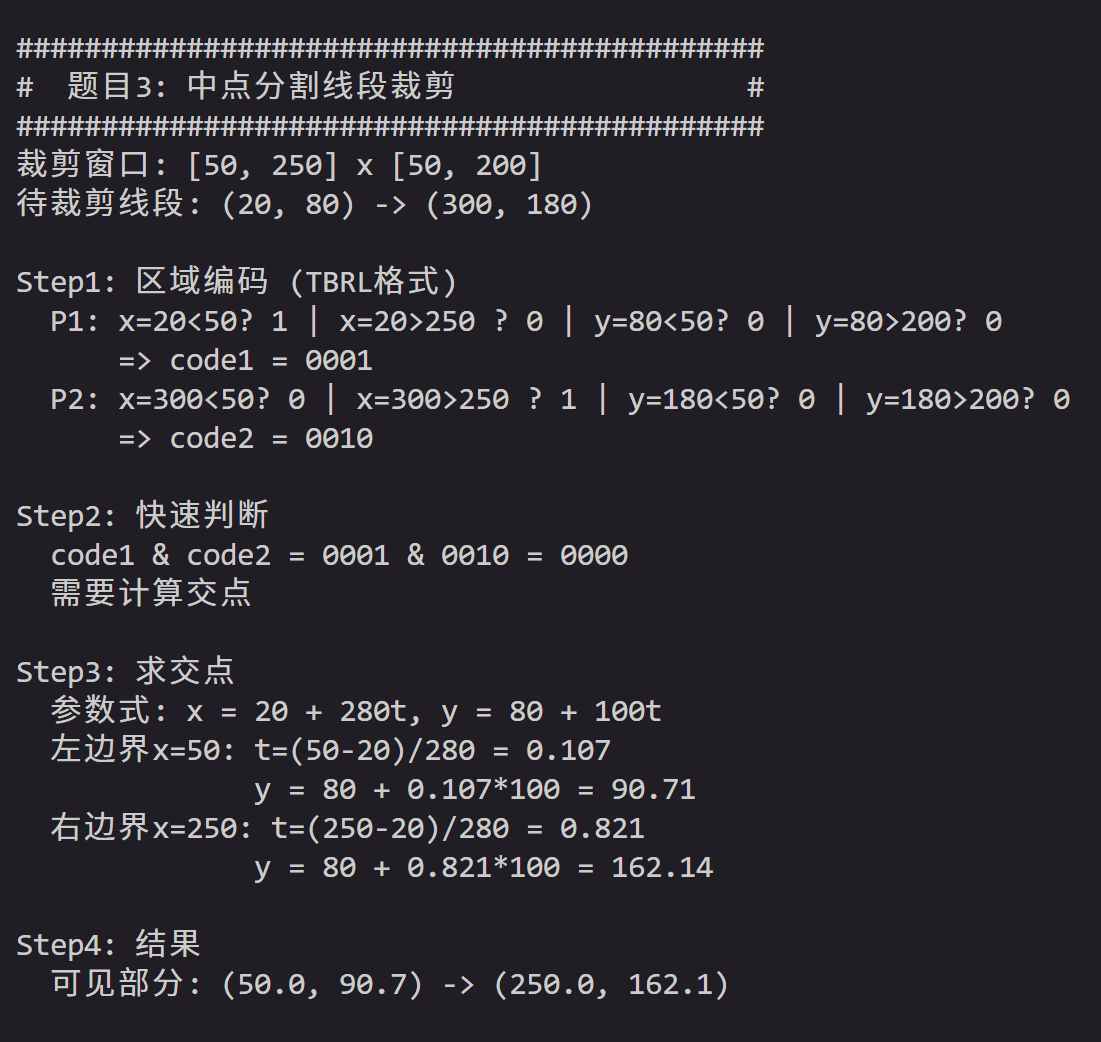
\includegraphics[width=0.8\textwidth]{midpoint_result.png}
    \caption{中点分割裁剪程序运行结果}
\end{figure}

\newpage
\section{Sutherland-Hodgman多边形裁剪算法}

\subsection{问题描述}
采用Sutherland-Hodgman算法实现矩形窗口ABCD对某多边形的裁剪。

\subsection{算法输入}
\begin{itemize}
    \item 待裁剪多边形：顶点序列 $\{P_1, P_2, ..., P_n\}$（按顺序连接）
    \item 矩形裁剪窗口：由 $(x_{min}, y_{min})$ 和 $(x_{max}, y_{max})$ 定义
\end{itemize}

\subsection{算法输出}
\begin{itemize}
    \item 裁剪后的多边形顶点序列 $\{V_1, V_2, ..., V_m\}$
    \item 若多边形完全在窗口外，返回空序列
\end{itemize}

\subsection{算法流程}
\begin{enumerate}
    \item \textbf{初始化}：将输入多边形作为当前多边形
    \item \textbf{依次对四条边裁剪}：按左、右、下、上的顺序处理每条裁剪边
    \item \textbf{单边裁剪过程}：对于当前裁剪边，遍历多边形的每条边 $(P_i, P_{i+1})$：
    \begin{enumerate}
        \item 判断 $P_i$ 和 $P_{i+1}$ 相对于裁剪边的位置（内侧/外侧）
        \item 根据四种情况决定输出：
        \begin{itemize}
            \item \textbf{情况1}：两点都在内侧 $\rightarrow$ 输出 $P_{i+1}$
            \item \textbf{情况2}：$P_i$在内侧，$P_{i+1}$在外侧 $\rightarrow$ 输出交点 $I$
            \item \textbf{情况3}：$P_i$在外侧，$P_{i+1}$在内侧 $\rightarrow$ 输出交点 $I$ 和 $P_{i+1}$
            \item \textbf{情况4}：两点都在外侧 $\rightarrow$ 不输出
        \end{itemize}
    \end{enumerate}
    \item \textbf{更新多边形}：将输出顶点序列作为下一条边的输入
    \item \textbf{返回结果}：四条边处理完毕后，返回最终的顶点序列
\end{enumerate}

\subsection{算法原理}
Sutherland-Hodgman算法依次用裁剪窗口的四条边对多边形进行裁剪，每次裁剪产生的新多边形作为下一次裁剪的输入。算法的核心是对每条边进行"流水线"式处理。

\subsection{Rust代码实现}

\begin{lstlisting}
#[derive(Debug, Clone, Copy)]
pub struct Point { pub x: f64, pub y: f64 }

#[derive(Debug, Clone, Copy)]
pub struct Rect { pub xmin: f64, pub ymin: f64, pub xmax: f64, pub ymax: f64 }

#[derive(Clone, Copy)]
pub enum Edge { Left, Right, Bottom, Top }

impl Rect {
    fn is_inside(&self, p: &Point, edge: Edge) -> bool {
        match edge {
            Edge::Left => p.x >= self.xmin,   Edge::Right => p.x <= self.xmax,
            Edge::Bottom => p.y >= self.ymin, Edge::Top => p.y <= self.ymax,
        }
    }

    fn intersect(&self, p1: &Point, p2: &Point, edge: Edge) -> Point {
        let (x1, y1, x2, y2) = (p1.x, p1.y, p2.x, p2.y);
        match edge {
            Edge::Left => {
                let t = (self.xmin - x1) / (x2 - x1);
                Point { x: self.xmin, y: y1 + t * (y2 - y1) }
            }
            Edge::Right => {
                let t = (self.xmax - x1) / (x2 - x1);
                Point { x: self.xmax, y: y1 + t * (y2 - y1) }
            }
            Edge::Bottom => {
                let t = (self.ymin - y1) / (y2 - y1);
                Point { x: x1 + t * (x2 - x1), y: self.ymin }
            }
            Edge::Top => {
                let t = (self.ymax - y1) / (y2 - y1);
                Point { x: x1 + t * (x2 - x1), y: self.ymax }
            }
        }
    }

    fn clip_edge(&self, polygon: &[Point], edge: Edge) -> Vec<Point> {
        let mut output = Vec::new();
        let n = polygon.len();
        for i in 0..n {
            let (curr, next) = (polygon[i], polygon[(i + 1) % n]);
            let (ci, ni) = (self.is_inside(&curr, edge), self.is_inside(&next, edge));
            match (ci, ni) {
                (true, true) => output.push(next),
                (true, false) => output.push(self.intersect(&curr, &next, edge)),
                (false, true) => {
                    output.push(self.intersect(&curr, &next, edge));
                    output.push(next);
                }
                _ => {}
            }
        }
        output
    }
}

pub fn sutherland_hodgman_clip(polygon: &[Point], rect: &Rect) -> Vec<Point> {
    let mut result = polygon.to_vec();
    for edge in [Edge::Left, Edge::Right, Edge::Bottom, Edge::Top] {
        result = rect.clip_edge(&result, edge);
        if result.is_empty() { break; }
    }
    result
}

fn main() {
    let rect = Rect { xmin: 80.0, ymin: 80.0, xmax: 280.0, ymax: 220.0 };
    let polygon = vec![
        Point { x: 30.0, y: 120.0 }, Point { x: 150.0, y: 30.0 },
        Point { x: 320.0, y: 100.0 }, Point { x: 300.0, y: 250.0 },
        Point { x: 180.0, y: 280.0 }, Point { x: 60.0, y: 200.0 },
    ];
    println!("窗口: x∈[{},{}], y∈[{},{}]", rect.xmin, rect.xmax, rect.ymin, rect.ymax);
    println!("多边形: {} 顶点", polygon.len());
    
    let clipped = sutherland_hodgman_clip(&polygon, &rect);
    println!("裁剪后: {} 顶点", clipped.len());
    for (i, p) in clipped.iter().enumerate() {
        println!("  V{}: ({:.1}, {:.1})", i+1, p.x, p.y);
    }
}
\end{lstlisting}

\subsection{算法执行过程示例}

以五边形$P_1(50,150), P_2(200,50), P_3(350,150), P_4(250,300), P_5(100,250)$为例，裁剪窗口为$(100,100)-(300,250)$：

\textbf{第一步：左边界裁剪（$x \geq 100$）}
\begin{itemize}
    \item $P_1 \to P_2$：$P_1$在外，$P_2$在内，输出交点$(100, 116.67)$和$P_2$
    \item $P_2 \to P_3$：两点都在内，输出$P_3$
    \item $P_3 \to P_4$：两点都在内，输出$P_4$
    \item $P_4 \to P_5$：两点都在内，输出$P_5$
    \item $P_5 \to P_1$：$P_5$在内，$P_1$在外，输出交点$(100, 250)$
\end{itemize}

\textbf{第二步：右边界裁剪（$x \leq 300$）}

\textbf{第三步：下边界裁剪（$y \geq 100$）}

\textbf{第四步：上边界裁剪（$y \leq 250$）}

最终得到裁剪后的多边形顶点序列。

\subsection{运行结果}
\begin{verbatim}
【输入数据】
  裁剪窗口W: x∈[100,300], y∈[100,250]
  多边形P: V1(50,150), V2(200,50), V3(350,150), V4(250,300), V5(100,250)
  原始面积 = 0.5*|Σ(xi*y(i+1) - x(i+1)*yi)| = 43750

【交点计算公式】
  线段(x1,y1)→(x2,y2)与边界的交点:
  - 垂直边x=k: t = (k-x1)/(x2-x1), y = y1 + t*(y2-y1)
  - 水平边y=k: t = (k-y1)/(y2-y1), x = x1 + t*(x2-x1)

【左边界裁剪 x≥100】
  V1(50,150)→V2(200,50): 外→内
    t = (100-50)/(200-50) = 50/150 = 1/3
    y = 150 + (1/3)*(50-150) = 150 - 100/3 = 116.67
    输出: 交点(100, 116.67), 终点V2
  V5(100,250)→V1(50,150): 内→外
    t = (100-100)/(50-100) = 0
    输出: 交点(100, 250)

【右边界裁剪 x≤300】
  V2(200,50)→V3(350,150): 内→外
    t = (300-200)/(350-200) = 100/150 = 2/3
    y = 50 + (2/3)*(150-50) = 50 + 200/3 = 116.67
    输出: 交点(300, 116.67)
  V3(350,150)→V4(250,300): 外→内
    t = (300-350)/(250-350) = -50/-100 = 0.5
    y = 150 + 0.5*(300-150) = 225
    输出: 交点(300, 225), 终点V4

【下边界裁剪 y≥100】
  (100,116.67)→(200,50): 内→外
    t = (100-116.67)/(50-116.67) = 0.25
    x = 100 + 0.25*(200-100) = 125
    输出: 交点(125, 100)
  (200,50)→(300,116.67): 外→内
    t = (100-50)/(116.67-50) = 0.75
    x = 200 + 0.75*(300-200) = 275
    输出: 交点(275, 100), 终点

【上边界裁剪 y≤250】
  (300,225)→(250,300): 内→外
    t = (250-225)/(300-225) = 25/75 = 1/3
    x = 300 + (1/3)*(250-300) = 283.33
    输出: 交点(283.33, 250)

【最终结果】
  裁剪后顶点: (300,116.67), (300,225), (283.33,250), (100,250),
              (100,116.67), (125,100), (275,100)
  裁剪后面积 = 29375
\end{verbatim}

\begin{figure}[H]
    \centering
    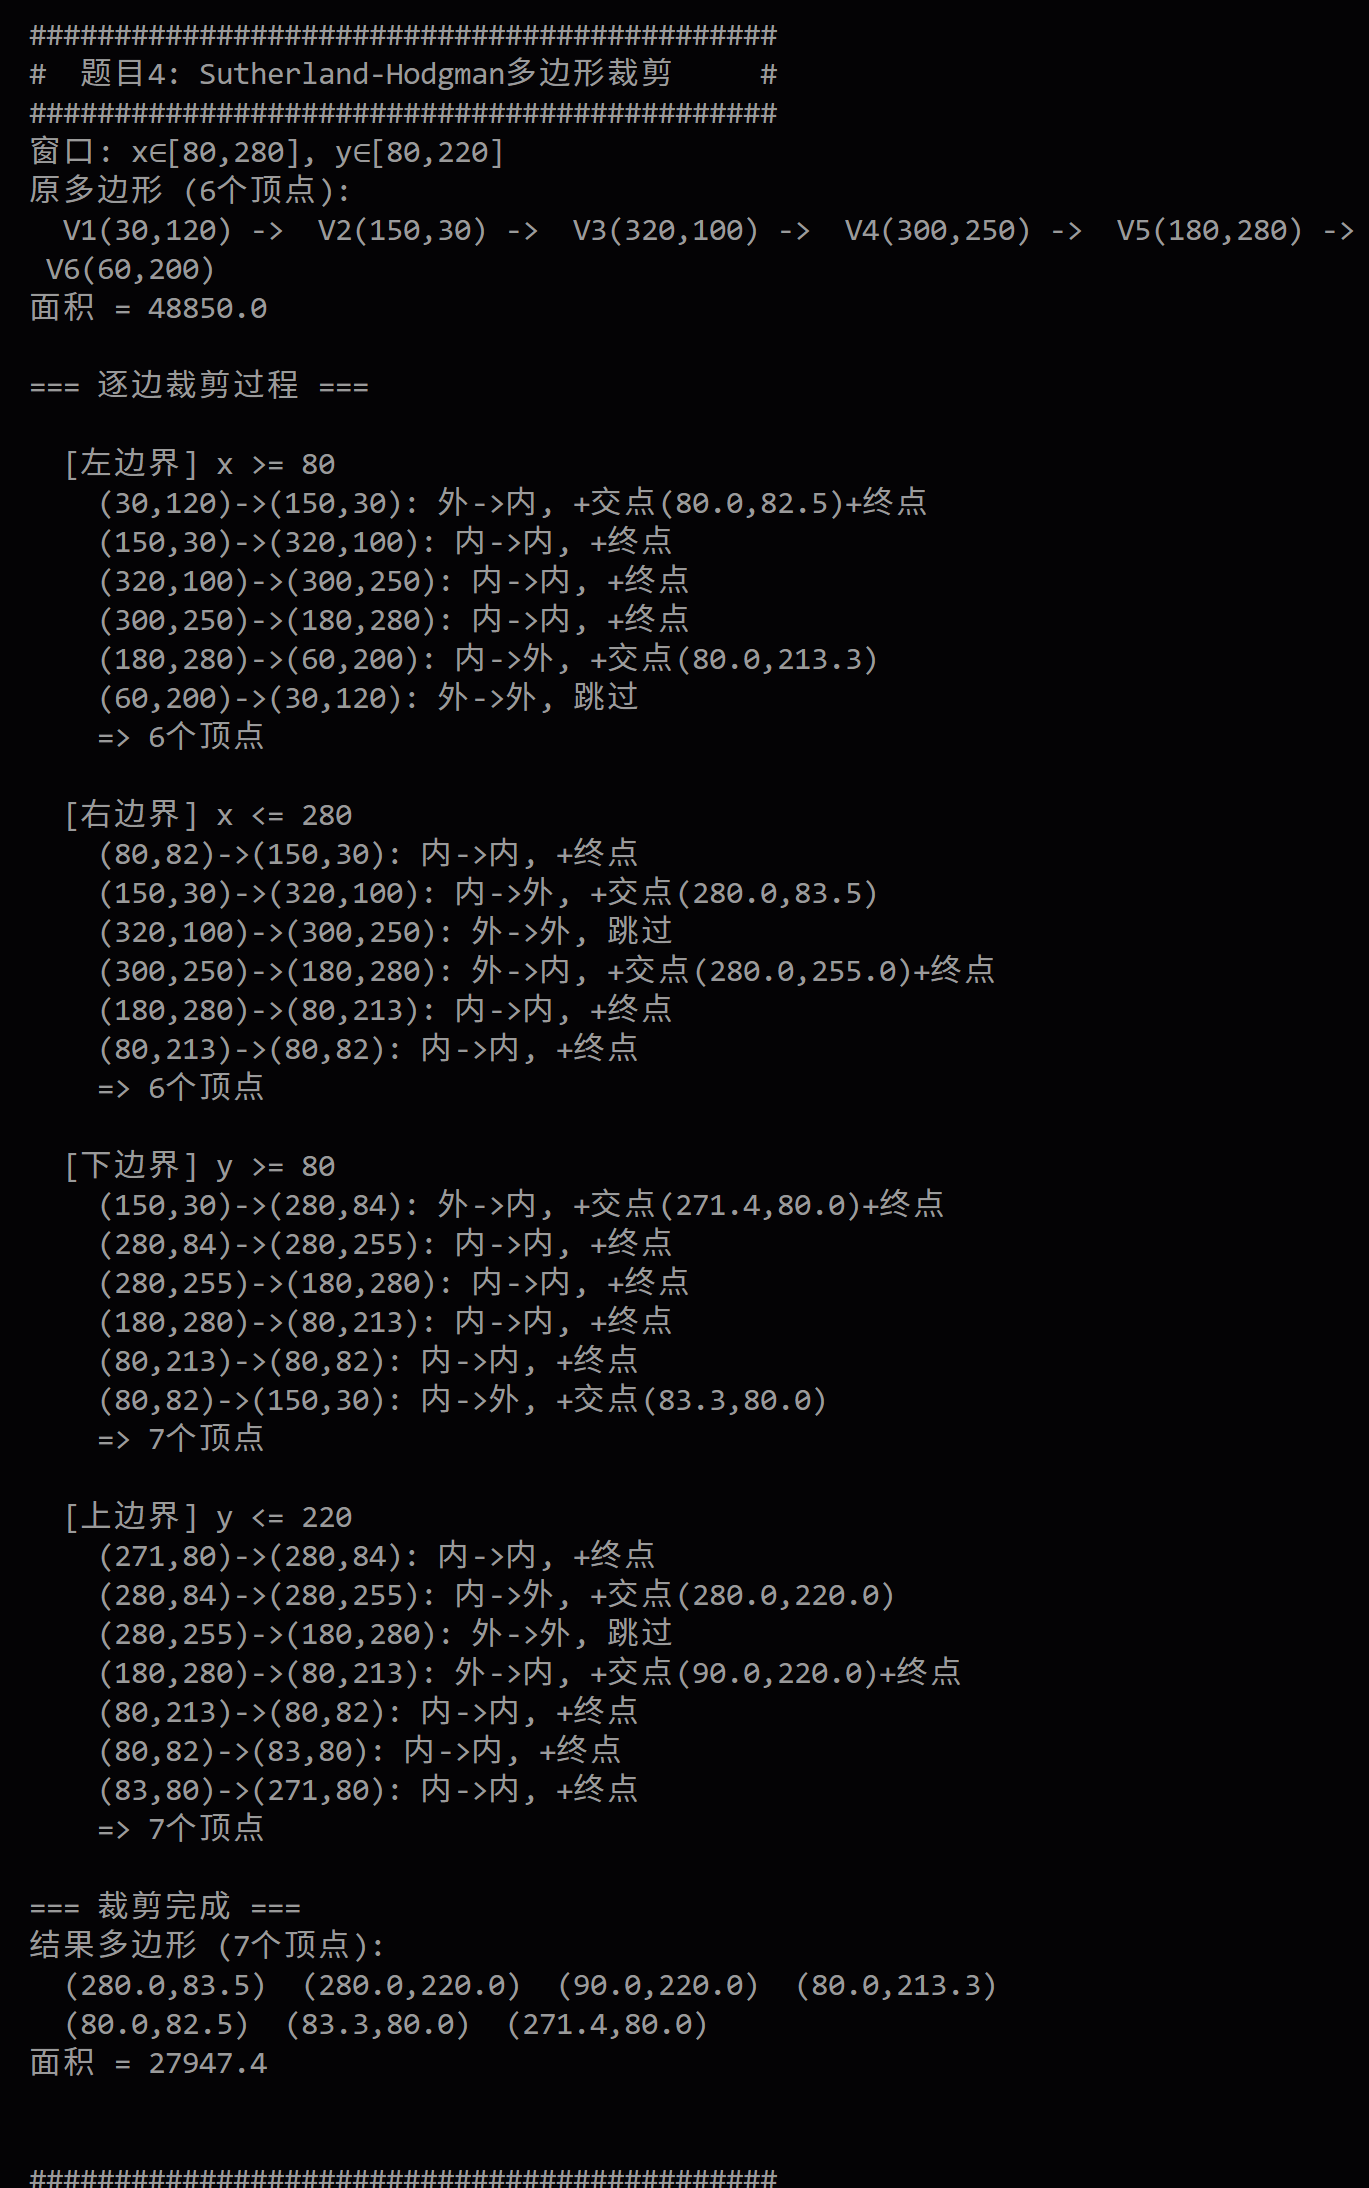
\includegraphics[width=0.8\textwidth]{sh_result.png}
    \caption{Sutherland-Hodgman多边形裁剪程序运行结果}
\end{figure}

\newpage
\section{Weiler-Atherton多边形裁剪算法}

\subsection{问题描述}
采用Weiler-Atherton算法实现多边形对多边形的裁剪。

\subsection{算法输入}
\begin{itemize}
    \item 主多边形（被裁剪多边形）：顶点序列 $S = \{S_1, S_2, ..., S_n\}$
    \item 裁剪多边形：顶点序列 $C = \{C_1, C_2, ..., C_m\}$
    \item 两个多边形均按相同方向（顺时针或逆时针）给出
\end{itemize}

\subsection{算法输出}
\begin{itemize}
    \item 裁剪结果多边形列表：$\{R_1, R_2, ..., R_k\}$（可能产生多个独立的多边形）
    \item 每个结果多边形为顶点序列
    \item 若无交集，返回空列表或包含的多边形
\end{itemize}

\subsection{算法流程}
\begin{enumerate}
    \item \textbf{计算所有交点}：
    \begin{enumerate}
        \item 遍历主多边形的每条边 $S_iS_{i+1}$
        \item 与裁剪多边形的每条边 $C_jC_{j+1}$ 求交
        \item 记录交点坐标、所在边的索引、参数位置 $t$
        \item 判断交点类型：检查交点后方向是否进入裁剪多边形内部
        \begin{itemize}
            \item 若进入内部：标记为"进入点"
            \item 若离开内部：标记为"离开点"
        \end{itemize}
    \end{enumerate}
    
    \item \textbf{处理特殊情况}：
    \begin{itemize}
        \item 若无交点且主多边形在裁剪多边形内：返回主多边形
        \item 若无交点且裁剪多边形在主多边形内：返回裁剪多边形
        \item 若无交点且不相交：返回空
    \end{itemize}
    
    \item \textbf{构建顶点链表}：
    \begin{enumerate}
        \item 将交点按参数 $t$ 排序后插入主多边形顶点链表
        \item 将交点按参数 $t$ 排序后插入裁剪多边形顶点链表
        \item 建立两个链表中对应交点的双向链接
    \end{enumerate}
    
    \item \textbf{遍历生成结果多边形}：
    \begin{enumerate}
        \item 找到一个未访问的"进入点"作为起点
        \item 沿主多边形链表前进，将顶点加入结果
        \item 遇到"离开点"时，通过链接切换到裁剪多边形链表
        \item 沿裁剪多边形链表前进
        \item 遇到"进入点"时，切换回主多边形链表
        \item 重复直到回到起点，完成一个结果多边形
        \item 继续查找其他未访问的进入点，生成更多结果多边形
    \end{enumerate}
    
    \item \textbf{返回结果}：返回所有生成的结果多边形列表
\end{enumerate}

\subsection{算法原理}
Weiler-Atherton算法是一种通用的多边形裁剪算法，可以处理凹多边形和带孔洞的多边形。

\textbf{核心思想：}基于交点链表，通过在进入点和离开点之间切换行走路径，生成裁剪结果。

\textbf{交点分类：}
\begin{itemize}
    \item \textbf{进入点}：沿主多边形边界行走时，从裁剪多边形外部进入内部的交点
    \item \textbf{离开点}：沿主多边形边界行走时，从裁剪多边形内部离开到外部的交点
\end{itemize}

\subsection{Rust代码实现}

\begin{lstlisting}
use std::f64::consts::PI;

#[derive(Debug, Clone, Copy, PartialEq)]
struct Point { x: f64, y: f64 }

impl Point {
    fn new(x: f64, y: f64) -> Self { Point { x, y } }
    
    fn distance_sq(&self, other: &Point) -> f64 {
        let dx = self.x - other.x;
        let dy = self.y - other.y;
        dx * dx + dy * dy
    }
}

/// 顶点节点
#[derive(Debug, Clone)]
struct Vertex {
    pt: Point,
    t: f64,              // 在边上的参数位置
    is_intersection: bool,
    is_entering: bool,   // true=进入点, false=离开点
    neighbor: Option<usize>, // 对应另一链表中的索引
}

impl Vertex {
    fn new(pt: Point) -> Self {
        Vertex { pt, t: 0.0, is_intersection: false, 
                 is_entering: false, neighbor: None }
    }
    
    fn intersection(pt: Point, t: f64, entering: bool) -> Self {
        Vertex { pt, t, is_intersection: true, 
                 is_entering: entering, neighbor: None }
    }
}
\end{lstlisting}

\begin{lstlisting}
/// 计算两线段交点
fn compute_intersection(a1: Point, a2: Point, b1: Point, b2: Point) 
    -> Option<(f64, f64, Point)> {
    let dax = a2.x - a1.x;
    let day = a2.y - a1.y;
    let dbx = b2.x - b1.x;
    let dby = b2.y - b1.y;
    let denom = dax * dby - day * dbx;
    
    if denom.abs() < 1e-10 { return None; } // 平行
    
    let dx = b1.x - a1.x;
    let dy = b1.y - a1.y;
    let ta = (dx * dby - dy * dbx) / denom;
    let tb = (dx * day - dy * dax) / denom;
    
    const EPS: f64 = 1e-7;
    if ta > EPS && ta < 1.0 - EPS && tb > EPS && tb < 1.0 - EPS {
        let pt = Point::new(a1.x + ta * dax, a1.y + ta * day);
        Some((ta, tb, pt))
    } else {
        None
    }
}

/// 判断点是否在多边形内部（射线法）
fn point_in_polygon(pt: &Point, polygon: &[Point]) -> bool {
    let mut count = 0;
    let n = polygon.len();
    for i in 0..n {
        let p1 = polygon[i];
        let p2 = polygon[(i + 1) % n];
        if (p1.y <= pt.y && p2.y > pt.y) || (p2.y <= pt.y && p1.y > pt.y) {
            let x = p1.x + (pt.y - p1.y) / (p2.y - p1.y) * (p2.x - p1.x);
            if pt.x < x { count += 1; }
        }
    }
    count % 2 == 1
}

/// 计算多边形有符号面积
fn signed_area(polygon: &[Point]) -> f64 {
    let mut area = 0.0;
    let n = polygon.len();
    for i in 0..n {
        let j = (i + 1) % n;
        area += polygon[i].x * polygon[j].y;
        area -= polygon[j].x * polygon[i].y;
    }
    area / 2.0
}
\end{lstlisting}

\begin{lstlisting}
/// Weiler-Atherton多边形裁剪算法
fn weiler_atherton_clip(subject: &[Point], clip: &[Point]) -> Vec<Vec<Point>> {
    let mut result = Vec::new();
    if subject.len() < 3 || clip.len() < 3 { return result; }

    // 步骤1：计算所有交点
    struct Intersection {
        pt: Point,
        subj_edge: usize,
        clip_edge: usize,
        t_subj: f64,
        t_clip: f64,
        entering: bool,
    }
    let mut intersections = Vec::new();

    for i in 0..subject.len() {
        let s1 = subject[i];
        let s2 = subject[(i + 1) % subject.len()];
        for j in 0..clip.len() {
            let c1 = clip[j];
            let c2 = clip[(j + 1) % clip.len()];
            if let Some((ts, tc, pt)) = compute_intersection(s1, s2, c1, c2) {
                // 判断进入/离开
                let after_pt = Point::new(
                    s1.x + (ts + 0.001) * (s2.x - s1.x),
                    s1.y + (ts + 0.001) * (s2.y - s1.y),
                );
                let entering = point_in_polygon(&after_pt, clip);
                intersections.push(Intersection {
                    pt, subj_edge: i, clip_edge: j,
                    t_subj: ts, t_clip: tc, entering,
                });
            }
        }
    }

    // 无交点的特殊情况
    if intersections.is_empty() {
        if point_in_polygon(&subject[0], clip) {
            result.push(subject.to_vec());
        } else if point_in_polygon(&clip[0], subject) {
            result.push(clip.to_vec());
        }
        return result;
    }

    // 步骤2：构建主多边形顶点链表
    let mut subj_list: Vec<Vertex> = Vec::new();
    for i in 0..subject.len() {
        subj_list.push(Vertex::new(subject[i]));
        let mut edge_inters: Vec<_> = intersections.iter()
            .filter(|inter| inter.subj_edge == i)
            .map(|inter| (inter.t_subj, inter))
            .collect();
        edge_inters.sort_by(|a, b| a.0.partial_cmp(&b.0).unwrap());
        for (t, inter) in edge_inters {
            subj_list.push(Vertex::intersection(inter.pt, t, inter.entering));
        }
    }
\end{lstlisting}

\begin{lstlisting}
    // 步骤3：构建裁剪多边形顶点链表
    let mut clip_list: Vec<Vertex> = Vec::new();
    for j in 0..clip.len() {
        clip_list.push(Vertex::new(clip[j]));
        let mut edge_inters: Vec<_> = intersections.iter()
            .filter(|inter| inter.clip_edge == j)
            .map(|inter| (inter.t_clip, inter))
            .collect();
        edge_inters.sort_by(|a, b| a.0.partial_cmp(&b.0).unwrap());
        for (t, inter) in edge_inters {
            clip_list.push(Vertex::intersection(inter.pt, t, inter.entering));
        }
    }

    // 步骤4：建立交点双向链接
    for i in 0..subj_list.len() {
        if subj_list[i].is_intersection {
            for j in 0..clip_list.len() {
                if clip_list[j].is_intersection {
                    if subj_list[i].pt.distance_sq(&clip_list[j].pt) < 1e-4 {
                        subj_list[i].neighbor = Some(j);
                        clip_list[j].neighbor = Some(i);
                        break;
                    }
                }
            }
        }
    }

    // 步骤5：从进入点遍历生成结果
    let mut used: Vec<bool> = vec![false; subj_list.len()];
    
    for start_idx in 0..subj_list.len() {
        if !subj_list[start_idx].is_intersection || 
           !subj_list[start_idx].is_entering || used[start_idx] {
            continue;
        }

        let mut polygon = Vec::new();
        let mut idx = start_idx;
        let mut on_subject = true;
        let max_iter = (subj_list.len() + clip_list.len()) * 3;

        for _ in 0..max_iter {
            if on_subject {
                let v = &subj_list[idx];
                polygon.push(v.pt);
                if v.is_intersection { used[idx] = true; }
                
                // 离开点：切换到裁剪多边形
                if v.is_intersection && !v.is_entering {
                    if let Some(neighbor) = v.neighbor {
                        idx = (neighbor + 1) % clip_list.len();
                        on_subject = false;
                        continue;
                    }
                }
                idx = (idx + 1) % subj_list.len();
                if idx == start_idx { break; }
            } else {
                let v = &clip_list[idx];
                // 进入点：切换回主多边形
                if v.is_intersection && v.neighbor.map_or(false, 
                    |n| subj_list[n].is_entering) {
                    if v.neighbor == Some(start_idx) { break; }
                    idx = v.neighbor.unwrap();
                    on_subject = true;
                    continue;
                }
                polygon.push(v.pt);
                idx = (idx + 1) % clip_list.len();
            }
        }

        if polygon.len() >= 3 {
            result.push(polygon);
        }
    }
    result
}
\end{lstlisting}

\begin{lstlisting}
fn main() {
    // 主多边形: 五边形
    let subject = vec![
        Point::new(80.0, 120.0), Point::new(220.0, 80.0),
        Point::new(320.0, 180.0), Point::new(260.0, 300.0),
        Point::new(100.0, 260.0),
    ];
    // 裁剪多边形: 矩形
    let clip = vec![
        Point::new(120.0, 100.0), Point::new(280.0, 100.0),
        Point::new(280.0, 250.0), Point::new(120.0, 250.0),
    ];

    println!("主多边形S: {} 顶点, 面积={:.0}", subject.len(), signed_area(&subject).abs());
    println!("裁剪多边形C: {} 顶点, 面积={:.0}", clip.len(), signed_area(&clip).abs());

    let results = weiler_atherton_clip(&subject, &clip);
    println!("裁剪结果: {} 个多边形", results.len());
    for (i, poly) in results.iter().enumerate() {
        println!("  多边形#{}: {} 顶点, 面积={:.1}", i+1, poly.len(), signed_area(poly).abs());
    }
}
\end{lstlisting}

\subsection{算法执行过程示例}

以正方形主多边形$S_1(100,100), S_2(300,100), S_3(300,300), S_4(100,300)$和菱形裁剪多边形$C_1(150,50), C_2(350,200), C_3(200,350), C_4(50,200)$为例：

\textbf{步骤1：计算交点}

计算主多边形和裁剪多边形所有边的交点，并判断每个交点是进入点还是离开点。

\textbf{步骤2：构建顶点链表}

将交点按参数顺序插入到两个多边形的顶点链表中。

\textbf{步骤3：遍历生成结果}

从第一个未访问的进入点开始，沿主多边形边界行走，遇到离开点时切换到裁剪多边形，遇到进入点时切换回主多边形，直到回到起点。

\subsection{运行结果}
\begin{verbatim}
【输入数据】
  主多边形S(正方形): S1(100,100), S2(300,100), S3(300,300), S4(100,300)
  面积 = 200×200 = 40000
  裁剪多边形C(菱形): C1(150,50), C2(350,200), C3(200,350), C4(50,200)
  面积 = 0.5×对角线乘积 = 0.5×300×300 = 45000

【交点计算公式】
  线段A1A2与B1B2的交点:
  设 P = A1 + ta*(A2-A1) = B1 + tb*(B2-B1)
  联立方程组:
    (A2x-A1x)*ta - (B2x-B1x)*tb = B1x - A1x
    (A2y-A1y)*ta - (B2y-B1y)*tb = B1y - A1y
  用克莱姆法则求解ta, tb

【交点详细计算】
  S1S2 × C4C1: S1(100,100)→S2(300,100), C4(50,200)→C1(150,50)
    方向向量: dS=(200,0), dC=(100,-150)
    行列式: D = 200×(-150) - 0×100 = -30000
    ta = [(50-100)×(-150) - (200-100)×100] / (-30000)
       = [7500 - 10000] / (-30000) = 1/12 ≈ 0.0833
    x = 100 + 0.0833×200 = 116.67, y = 100
    交点(116.67, 100), 类型: 进入点

  S1S2 × C1C2: S1(100,100)→S2(300,100), C1(150,50)→C2(350,200)
    dS=(200,0), dC=(200,150)
    D = 200×150 - 0×200 = 30000
    ta = [(150-100)×150 - (50-100)×200] / 30000
       = [7500 + 10000] / 30000 = 7/12 ≈ 0.5833
    x = 100 + 0.5833×200 = 216.67, y = 100
    交点(216.67, 100), 类型: 离开点

  S2S3 × C1C2: S2(300,100)→S3(300,300), C1(150,50)→C2(350,200)
    dS=(0,200), dC=(200,150)
    D = 0×150 - 200×200 = -40000
    ta = [(150-300)×150 - (50-100)×200] / (-40000)
       = [-22500 + 10000] / (-40000) = 0.3125
    y = 100 + 0.3125×200 = 162.5
    交点(300, 162.5), 类型: 进入点

  S2S3 × C2C3: ta = 0.75, 交点(300, 250), 离开点
  S3S4 × C2C3: ta = 0.25, 交点(250, 300), 进入点
  S3S4 × C3C4: ta = 0.75, 交点(150, 300), 离开点
  S4S1 × C3C4: ta = 0.25, 交点(100, 250), 进入点
  S4S1 × C4C1: ta = 0.875, 交点(100, 125), 离开点

  共8个交点: 4个进入点, 4个离开点

【遍历生成结果】
  从进入点(116.67,100)出发，沿S边界前进:
  (116.67,100)[IN] → (216.67,100)[OUT] → 切换到C
  沿C边界 → (300,162.5)[IN] → 切换回S
  (300,162.5) → (300,250)[OUT] → 切换到C
  沿C边界 → (250,300)[IN] → 切换回S
  ... 继续直到回到起点

【最终结果】
  裁剪后顶点(8个):
    (116.67,100), (216.67,100), (300,162.5), (300,250),
    (250,300), (150,300), (100,250), (100,125)
  裁剪后面积 = 34687.5
\end{verbatim}

\begin{figure}[H]
    \centering
    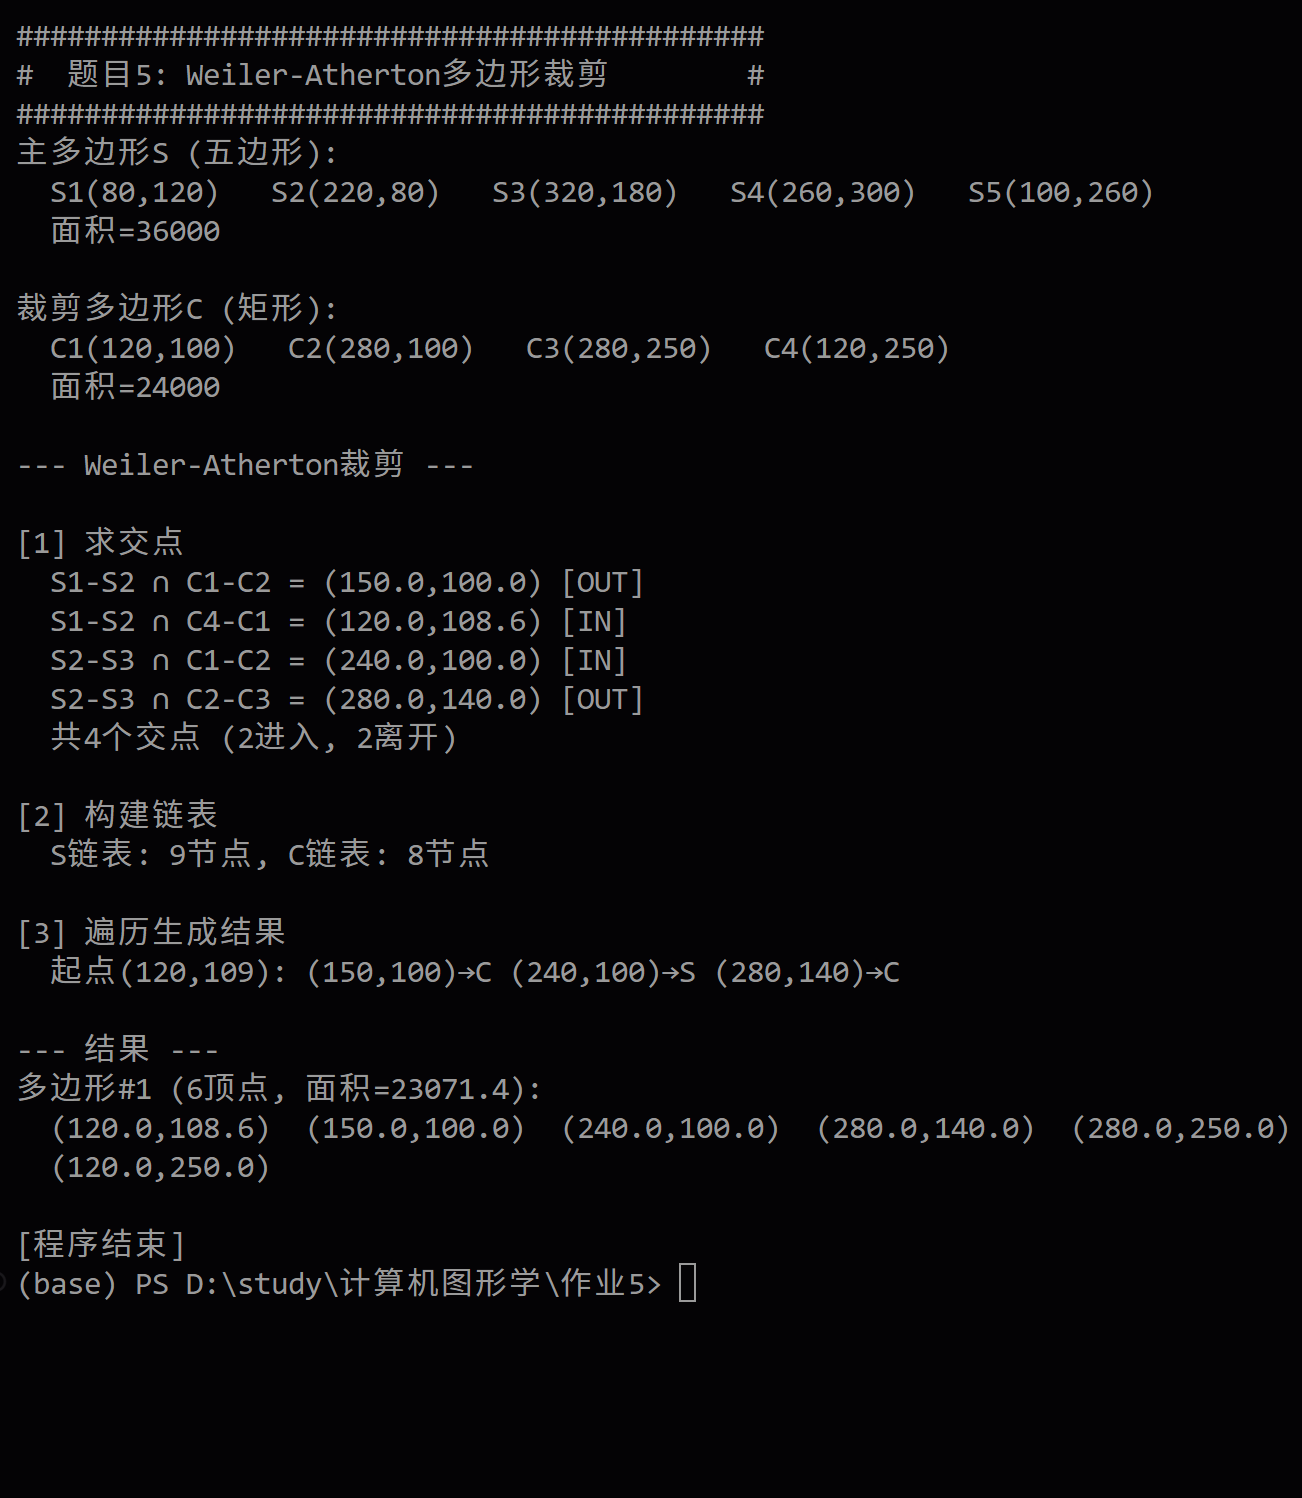
\includegraphics[width=0.8\textwidth]{wa_result.png}
    \caption{Weiler-Atherton多边形裁剪程序运行结果}
\end{figure}

\end{document}
